\chapter{\rm\bfseries Probabilistic Program Repair}
\label{ch:chapter03}

As we have seen, the problem of program repair is highly underdetermined. To resolve this ambiguity, we will use a probabilistic model to induce a distribution over the language of valid programs. This distribution will guide the repair process by assigning a likelihood to each possible repair. Then, taking the maximum over all possible repairs, we can find the most likely repair consistent with the constraints and the observed program.

Specifically, we will define an ordering over strings by their likelihood under the probabilistic model. We then define a repair as the most likely string consistent with the observed program and the grammar. We factorize the probability of a string as the product of the probability of each token in the string, conditioned on its predecessors. This allows us to compute the joint probability in a left-to-right fashion.

This probabilistic model will generally admit programs that are locally probable, but globally inconsistent with the grammar. To enforce syntactic validity, we will use the probabilistic language model to ``steer'' a generative sampler through the automaton representing the repair language. This has two advantages: first, it allows us to sample from the repair language incrementally, and second, it ensures that subsequences with high probability are retrieved first, and all trajectories are syntactically valid.

We will consider two kinds of probabilistic models: a constrained Markov model and an unconstrained transformer-based neural network trained on program repair, then evaluate the performance of these models on a syntax repair benchmark consisting of pairwise program transformations. As we will show, the constrained Markov model is able to achieve state-of-the-art precision on blind prediction of the lexical sequence.

Here we give each model 5k+ syntax repairs of varying lengths and Levenshtein distances and measure the precision at varying cutoffs. For example, if the ground truth syntax repair was contained in the top 10 results for half of the repair instances, the model's P@10 would be 50\%.

\begin{figure}[H]
  \resizebox{.24\textwidth}{!}{\input{../popl2025/len_dist_tidy}}
  \resizebox{.24\textwidth}{!}{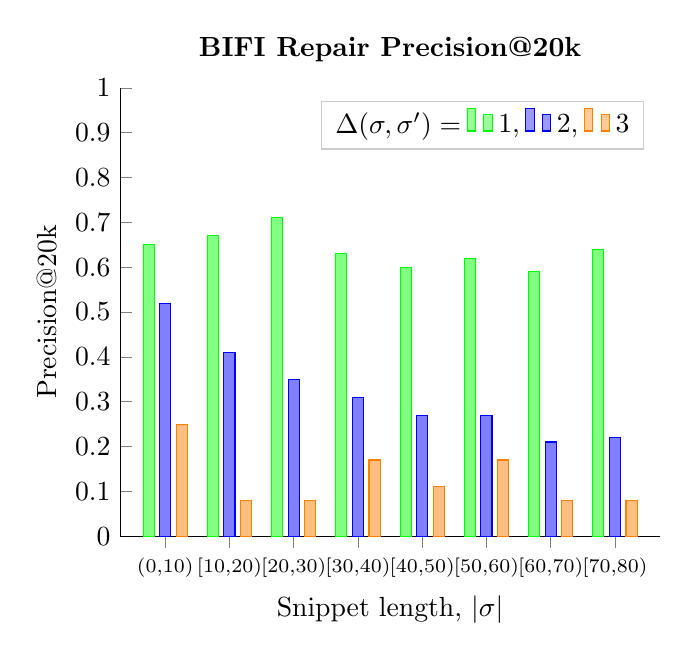
\begin{tikzpicture}
  \begin{axis}[
  xlabel={Snippet length, $|\sigma|$},
  ylabel={Precision@20k},
  title={\textbf{BIFI Repair Precision@20k}},
  legend cell align={left},
  legend style={fill opacity=0.8, draw opacity=1, text opacity=1, draw=lightgray204, legend columns=-1, legend pos=north east},
  ybar,
  axis lines*=left,
  xtick={0, 10, 20, 30, 40, 50, 60, 70},
  ytick={0, 0.1, 0.2, 0.3, 0.4, 0.5, 0.6, 0.7, 0.8, 0.9, 1.0},
  xticklabels={{(}0{,}10{)}, {[}10{,}20{)}, {[}20{,}30{)}, {[}30{,}40{)}, {[}40{,}50{)}, {[}50{,}60{)}, {[}60{,}70{)}, {[}70{,}80{)}},
  x tick label style={font=\scriptsize},
  ymax=1.0,
  ymin=0.0,
  bar width=4pt,
  ]

  \addlegendimage{empty legend}
  \addlegendentry{$\Delta(\err\sigma, \sigma')=$}
  \addlegendimage{ybar,ybar legend,draw=none,green,fill=green!50}
  \addlegendentry{1,}
  \addlegendimage{ybar,ybar legend,draw=none,blue,fill=blue!50}
  \addlegendentry{2,}
  \addlegendimage{ybar,ybar legend,draw=none,orange,fill=orange!50}
  \addlegendentry{3}

  \addplot[green, fill=green!50] coordinates   {(0, 0.65) (10, 0.67) (20, 0.71) (30, 0.63) (40, 0.60) (50, 0.62) (60, 0.59) (70, 0.64)};
  \addplot[blue, fill=blue!50] coordinates     {(0, 0.52) (10, 0.41) (20, 0.35) (30, 0.31) (40, 0.27) (50, 0.27) (60, 0.21) (70, 0.22)};
  \addplot[orange, fill=orange!50] coordinates {(0, 0.25) (10, 0.08) (20, 0.08) (30, 0.17) (40, 0.11) (50, 0.17) (60, 0.08) (70, 0.08)};

  \end{axis}
\end{tikzpicture}
}
  \resizebox{.24\textwidth}{!}{\input{../popl2025/len_dist_s2p}}
  \resizebox{.24\textwidth}{!}{\input{../popl2025/len_dist_bifi}}
  \caption{Total repair precision across the entire test set.}
\end{figure}

If we give it an equivalent number of samples, the constrained Markov model attains an even wider margin.

\begin{figure}[H]
  \resizebox{.24\textwidth}{!}{\input{../popl2025/len_dist_tidy}}
  \resizebox{.24\textwidth}{!}{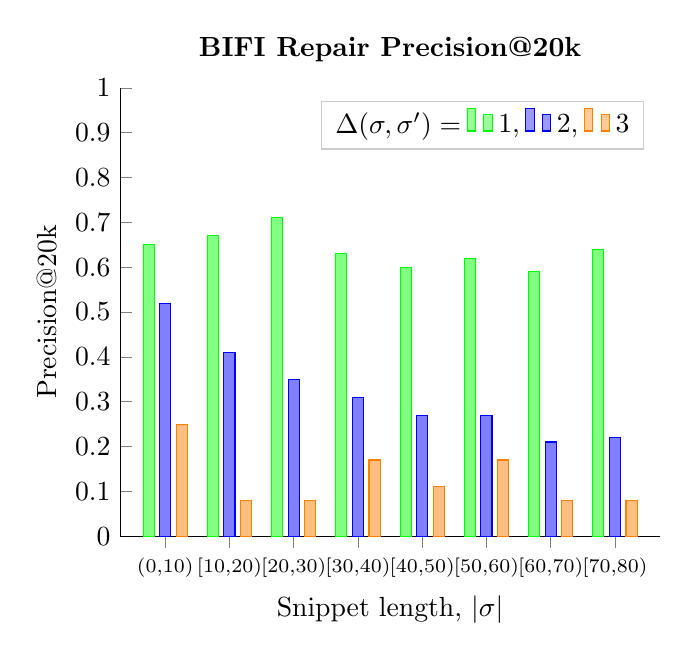
\begin{tikzpicture}
  \begin{axis}[
  xlabel={Snippet length, $|\sigma|$},
  ylabel={Precision@20k},
  title={\textbf{BIFI Repair Precision@20k}},
  legend cell align={left},
  legend style={fill opacity=0.8, draw opacity=1, text opacity=1, draw=lightgray204, legend columns=-1, legend pos=north east},
  ybar,
  axis lines*=left,
  xtick={0, 10, 20, 30, 40, 50, 60, 70},
  ytick={0, 0.1, 0.2, 0.3, 0.4, 0.5, 0.6, 0.7, 0.8, 0.9, 1.0},
  xticklabels={{(}0{,}10{)}, {[}10{,}20{)}, {[}20{,}30{)}, {[}30{,}40{)}, {[}40{,}50{)}, {[}50{,}60{)}, {[}60{,}70{)}, {[}70{,}80{)}},
  x tick label style={font=\scriptsize},
  ymax=1.0,
  ymin=0.0,
  bar width=4pt,
  ]

  \addlegendimage{empty legend}
  \addlegendentry{$\Delta(\err\sigma, \sigma')=$}
  \addlegendimage{ybar,ybar legend,draw=none,green,fill=green!50}
  \addlegendentry{1,}
  \addlegendimage{ybar,ybar legend,draw=none,blue,fill=blue!50}
  \addlegendentry{2,}
  \addlegendimage{ybar,ybar legend,draw=none,orange,fill=orange!50}
  \addlegendentry{3}

  \addplot[green, fill=green!50] coordinates   {(0, 0.65) (10, 0.67) (20, 0.71) (30, 0.63) (40, 0.60) (50, 0.62) (60, 0.59) (70, 0.64)};
  \addplot[blue, fill=blue!50] coordinates     {(0, 0.52) (10, 0.41) (20, 0.35) (30, 0.31) (40, 0.27) (50, 0.27) (60, 0.21) (70, 0.22)};
  \addplot[orange, fill=orange!50] coordinates {(0, 0.25) (10, 0.08) (20, 0.08) (30, 0.17) (40, 0.11) (50, 0.17) (60, 0.08) (70, 0.08)};

  \end{axis}
\end{tikzpicture}
}
  \resizebox{.24\textwidth}{!}{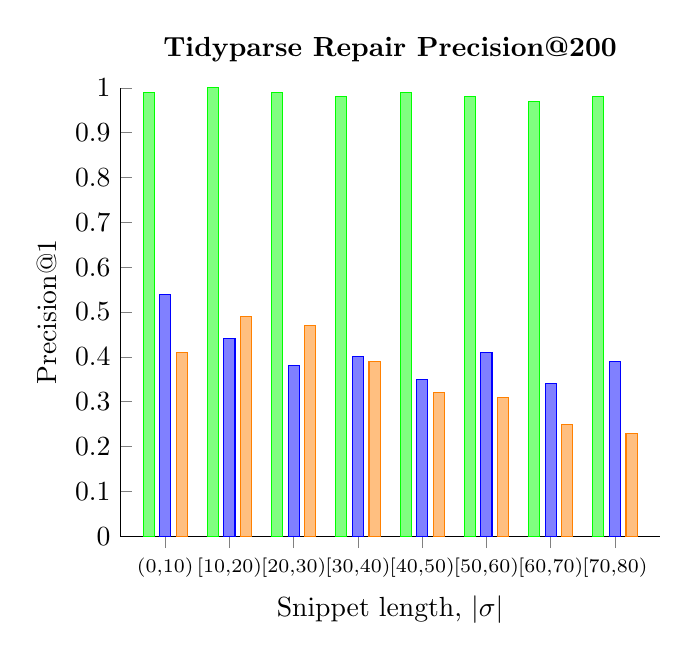
\begin{tikzpicture}
  \begin{axis}[
    xlabel={Snippet length, $|\sigma|$},
    ylabel={Precision@1},
    title={\textbf{Tidyparse Repair Precision@200}},
    ybar,
    axis lines*=left,
    xtick={0, 10, 20, 30, 40, 50, 60, 70},
    ytick={0, 0.1, 0.2, 0.3, 0.4, 0.5, 0.6, 0.7, 0.8, 0.9, 1.0},
    xticklabels={{(}0{,}10{)}, {[}10{,}20{)}, {[}20{,}30{)}, {[}30{,}40{)}, {[}40{,}50{)}, {[}50{,}60{)}, {[}60{,}70{)}, {[}70{,}80{)}},
    x tick label style={font=\scriptsize},
    ymax=1.0,
    ymin=0.0,
    bar width=4pt,
  ]

  \addplot[green, fill=green!50] coordinates   {(0, 0.99) (10, 1.00) (20, 0.99) (30, 0.98) (40, 0.99) (50, 0.98) (60, 0.97) (70, 0.98)};
  \addplot[blue, fill=blue!50] coordinates     {(0, 0.54) (10, 0.44) (20, 0.38) (30, 0.40) (40, 0.35) (50, 0.41) (60, 0.34) (70, 0.39)};
  \addplot[orange, fill=orange!50] coordinates {(0, 0.41) (10, 0.49) (20, 0.47) (30, 0.39) (40, 0.32) (50, 0.31) (60, 0.25) (70, 0.23)};

  \end{axis}
\end{tikzpicture}

%                                    TIDY-GWA                     TIDY-CFG                  TIDY-ENUM
%(|σ|∈[0, 10), Δ=1): Top-1/total:    56 / 100 = 0.56               54 / 99 = 0.55            57 / 100 = 0.57
%(|σ|∈[0, 10), Δ=2): Top-1/total:    37 / 100 = 0.37              19 / 100 = 0.19            22 / 100 = 0.22
%(|σ|∈[0, 10), Δ=3): Top-1/total:      9 / 50 = 0.18                6 / 50 = 0.12              6 / 50 = 0.12

%(|σ|∈[10, 20), Δ=1): Top-1/total:   44 / 100 = 0.44              42 / 100 = 0.42            45 / 100 = 0.45
%(|σ|∈[10, 20), Δ=2): Top-1/total:   28 / 100 = 0.28              13 / 100 = 0.13            14 / 100 = 0.14
%(|σ|∈[10, 20), Δ=3): Top-1/total:   20 / 100 = 0.20               9 / 100 = 0.09             8 / 100 = 0.08

%(|σ|∈[20, 30), Δ=1): Top-1/total:   43 / 100 = 0.43              49 / 100 = 0.49            49 / 100 = 0.49
%(|σ|∈[20, 30), Δ=2): Top-1/total:   26 / 100 = 0.26              13 / 100 = 0.13            18 / 100 = 0.18
%(|σ|∈[20, 30), Δ=3): Top-1/total:    19 / 99 = 0.19                8 / 99 = 0.08              8 / 99 = 0.08

%(|σ|∈[30, 40), Δ=1): Top-1/total:   49 / 100 = 0.49              43 / 100 = 0.43            48 / 100 = 0.48
%(|σ|∈[30, 40), Δ=2): Top-1/total:   24 / 100 = 0.24              15 / 100 = 0.15            18 / 100 = 0.18
%(|σ|∈[30, 40), Δ=3): Top-1/total:   15 / 100 = 0.15              10 / 100 = 0.10             6 / 100 = 0.06

%(|σ|∈[40, 50), Δ=1): Top-1/total:   55 / 100 = 0.55              56 / 100 = 0.56            57 / 100 = 0.57
%(|σ|∈[40, 50), Δ=2): Top-1/total:   19 / 100 = 0.19              21 / 100 = 0.21            18 / 100 = 0.18
%(|σ|∈[40, 50), Δ=3): Top-1/total:   10 / 100 = 0.10               8 / 100 = 0.08             5 / 100 = 0.05

%(|σ|∈[50, 60), Δ=1): Top-1/total:   55 / 100 = 0.55              67 / 100 = 0.67            53 / 100 = 0.53
%(|σ|∈[50, 60), Δ=2): Top-1/total:   25 / 100 = 0.25              16 / 100 = 0.16            21 / 100 = 0.21
%(|σ|∈[50, 60), Δ=3): Top-1/total:    9 / 100 = 0.09               9 / 100 = 0.09             7 / 100 = 0.07

%(|σ|∈[60, 70), Δ=1): Top-1/total:   53 / 100 = 0.53              56 / 100 = 0.56            60 / 100 = 0.60
%(|σ|∈[60, 70), Δ=2): Top-1/total:   23 / 100 = 0.23              15 / 100 = 0.15            10 / 100 = 0.10
%(|σ|∈[60, 70), Δ=3): Top-1/total:   11 / 100 = 0.11               5 / 100 = 0.05             2 / 100 = 0.02

%(|σ|∈[70, 80), Δ=1): Top-1/total:   57 / 100 = 0.57              62 / 100 = 0.62            63 / 100 = 0.63
%(|σ|∈[70, 80), Δ=2): Top-1/total:   18 / 100 = 0.18              12 / 100 = 0.12            15 / 100 = 0.15
%(|σ|∈[70, 80), Δ=3): Top-1/total:     9 / 81 = 0.11                4 / 81 = 0.05              3 / 81 = 0.04}
  \resizebox{.24\textwidth}{!}{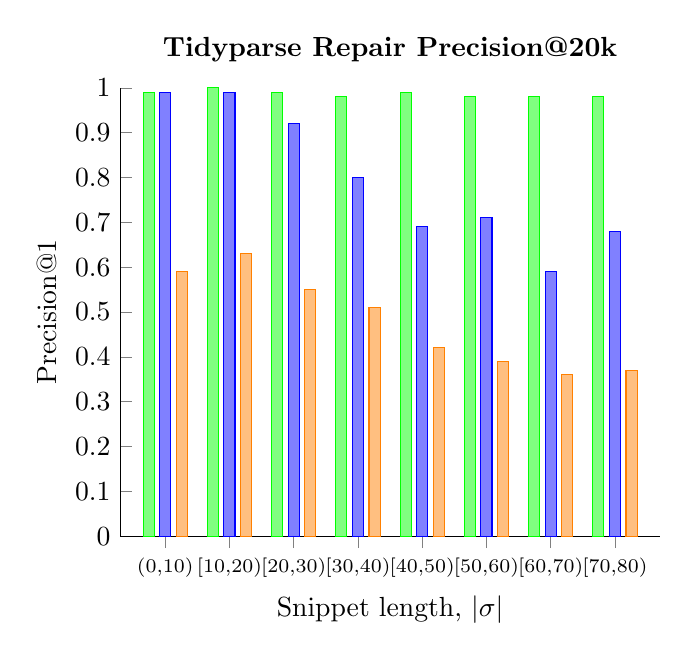
\begin{tikzpicture}
  \begin{axis}[
    xlabel={Snippet length, $|\sigma|$},
    ylabel={Precision@1},
    title={\textbf{Tidyparse Repair Precision@20k}},
    ybar,
    axis lines*=left,
    xtick={0, 10, 20, 30, 40, 50, 60, 70},
    ytick={0, 0.1, 0.2, 0.3, 0.4, 0.5, 0.6, 0.7, 0.8, 0.9, 1.0},
    xticklabels={{(}0{,}10{)}, {[}10{,}20{)}, {[}20{,}30{)}, {[}30{,}40{)}, {[}40{,}50{)}, {[}50{,}60{)}, {[}60{,}70{)}, {[}70{,}80{)}},
    x tick label style={font=\scriptsize},
    ymax=1.0,
    ymin=0.0,
    bar width=4pt,
  ]

  \addplot[green, fill=green!50] coordinates   {(0, 0.99) (10, 1.00) (20, 0.99) (30, 0.98) (40, 0.99) (50, 0.98) (60, 0.98) (70, 0.98)};
  \addplot[blue, fill=blue!50] coordinates     {(0, 0.99) (10, 0.99) (20, 0.92) (30, 0.80) (40, 0.69) (50, 0.71) (60, 0.59) (70, 0.68)};
  \addplot[orange, fill=orange!50] coordinates {(0, 0.59) (10, 0.63) (20, 0.55) (30, 0.51) (40, 0.42) (50, 0.39) (60, 0.36) (70, 0.37)};

  \end{axis}
\end{tikzpicture}

%                                    TIDY-GWA                     TIDY-CFG                  TIDY-ENUM
%(|σ|∈[0, 10), Δ=1): Top-1/total:    56 / 100 = 0.56               54 / 99 = 0.55            57 / 100 = 0.57
%(|σ|∈[0, 10), Δ=2): Top-1/total:    37 / 100 = 0.37              19 / 100 = 0.19            22 / 100 = 0.22
%(|σ|∈[0, 10), Δ=3): Top-1/total:      9 / 50 = 0.18                6 / 50 = 0.12              6 / 50 = 0.12

%(|σ|∈[10, 20), Δ=1): Top-1/total:   44 / 100 = 0.44              42 / 100 = 0.42            45 / 100 = 0.45
%(|σ|∈[10, 20), Δ=2): Top-1/total:   28 / 100 = 0.28              13 / 100 = 0.13            14 / 100 = 0.14
%(|σ|∈[10, 20), Δ=3): Top-1/total:   20 / 100 = 0.20               9 / 100 = 0.09             8 / 100 = 0.08

%(|σ|∈[20, 30), Δ=1): Top-1/total:   43 / 100 = 0.43              49 / 100 = 0.49            49 / 100 = 0.49
%(|σ|∈[20, 30), Δ=2): Top-1/total:   26 / 100 = 0.26              13 / 100 = 0.13            18 / 100 = 0.18
%(|σ|∈[20, 30), Δ=3): Top-1/total:    19 / 99 = 0.19                8 / 99 = 0.08              8 / 99 = 0.08

%(|σ|∈[30, 40), Δ=1): Top-1/total:   49 / 100 = 0.49              43 / 100 = 0.43            48 / 100 = 0.48
%(|σ|∈[30, 40), Δ=2): Top-1/total:   24 / 100 = 0.24              15 / 100 = 0.15            18 / 100 = 0.18
%(|σ|∈[30, 40), Δ=3): Top-1/total:   15 / 100 = 0.15              10 / 100 = 0.10             6 / 100 = 0.06

%(|σ|∈[40, 50), Δ=1): Top-1/total:   55 / 100 = 0.55              56 / 100 = 0.56            57 / 100 = 0.57
%(|σ|∈[40, 50), Δ=2): Top-1/total:   19 / 100 = 0.19              21 / 100 = 0.21            18 / 100 = 0.18
%(|σ|∈[40, 50), Δ=3): Top-1/total:   10 / 100 = 0.10               8 / 100 = 0.08             5 / 100 = 0.05

%(|σ|∈[50, 60), Δ=1): Top-1/total:   55 / 100 = 0.55              67 / 100 = 0.67            53 / 100 = 0.53
%(|σ|∈[50, 60), Δ=2): Top-1/total:   25 / 100 = 0.25              16 / 100 = 0.16            21 / 100 = 0.21
%(|σ|∈[50, 60), Δ=3): Top-1/total:    9 / 100 = 0.09               9 / 100 = 0.09             7 / 100 = 0.07

%(|σ|∈[60, 70), Δ=1): Top-1/total:   53 / 100 = 0.53              56 / 100 = 0.56            60 / 100 = 0.60
%(|σ|∈[60, 70), Δ=2): Top-1/total:   23 / 100 = 0.23              15 / 100 = 0.15            10 / 100 = 0.10
%(|σ|∈[60, 70), Δ=3): Top-1/total:   11 / 100 = 0.11               5 / 100 = 0.05             2 / 100 = 0.02

%(|σ|∈[70, 80), Δ=1): Top-1/total:   57 / 100 = 0.57              62 / 100 = 0.62            63 / 100 = 0.63
%(|σ|∈[70, 80), Δ=2): Top-1/total:   18 / 100 = 0.18              12 / 100 = 0.12            15 / 100 = 0.15
%(|σ|∈[70, 80), Δ=3): Top-1/total:     9 / 81 = 0.11                4 / 81 = 0.05              3 / 81 = 0.04}
  \caption{Sample efficiency increases sharply at larger precision intervals.}
\end{figure}

Next, we measure latency, which attains state-of-the-art precision at about 10 seconds, and additional time results in higher precision.

\begin{figure}[H]
  \begin{center}
%    \resizebox{.19\textwidth}{!}{\input{bar_hillel_repair.tex}}
  \resizebox{.24\textwidth}{!}{% This file was created with tikzplotlib v0.10.1.
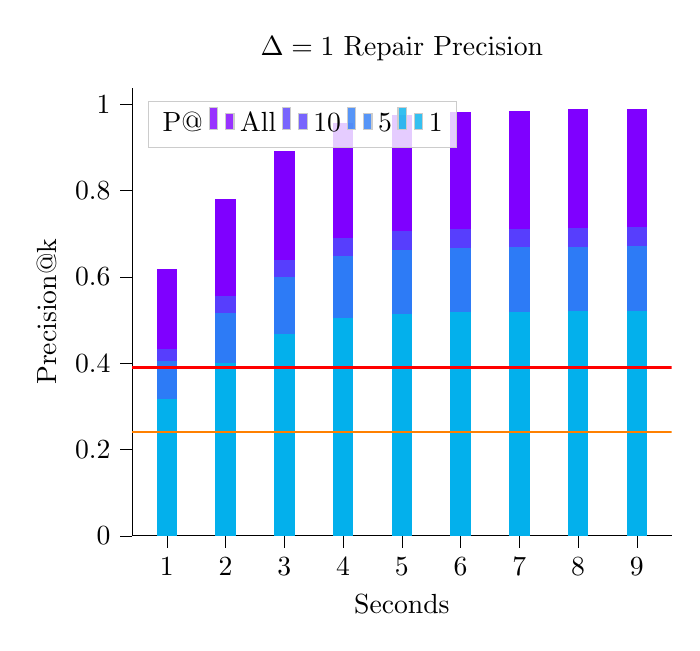
\begin{tikzpicture}
\begin{axis}[
legend cell align={left},
legend style={fill opacity=0.8, draw opacity=1, text opacity=1, draw=lightgray204, legend columns=-1, legend pos=north west},
tick align=outside,
tick pos=left,
axis lines*=left,
title={\(\displaystyle \Delta=1\) Repair Precision},
x grid style={darkgray176},
xlabel={Seconds},
xmin=-0.5925, xmax=8.5925,
xtick style={color=black},
xtick={0,1,2,3,4,5,6,7,8},
xticklabels={1,2,3,4,5,6,7,8,9},
y grid style={darkgray176},
ylabel={Precision@k},
ymin=0, ymax=1.03845,
ytick style={color=black}
]
\draw[draw=none,fill=darkviolet1270255] (axis cs:-0.175,0) rectangle (axis cs:0.175,0.619);
\addlegendimage{empty legend}
\addlegendentry{P@}
\addlegendimage{ybar,ybar legend,draw=none,fill=darkviolet1270255}
\addlegendentry{All}

\draw[draw=none,fill=darkviolet1270255] (axis cs:0.825,0) rectangle (axis cs:1.175,0.781);
\draw[draw=none,fill=darkviolet1270255] (axis cs:1.825,0) rectangle (axis cs:2.175,0.891);
\draw[draw=none,fill=darkviolet1270255] (axis cs:2.825,0) rectangle (axis cs:3.175,0.956);
\draw[draw=none,fill=darkviolet1270255] (axis cs:3.825,0) rectangle (axis cs:4.175,0.976);
\draw[draw=none,fill=darkviolet1270255] (axis cs:4.825,0) rectangle (axis cs:5.175,0.982);
\draw[draw=none,fill=darkviolet1270255] (axis cs:5.825,0) rectangle (axis cs:6.175,0.985);
\draw[draw=none,fill=darkviolet1270255] (axis cs:6.825,0) rectangle (axis cs:7.175,0.988);
\draw[draw=none,fill=darkviolet1270255] (axis cs:7.825,0) rectangle (axis cs:8.175,0.989);
\draw[draw=none,fill=royalblue8762253] (axis cs:-0.175,0) rectangle (axis cs:0.175,0.434);
\addlegendimage{ybar,ybar legend,draw=none,fill=royalblue8762253}
\addlegendentry{10}

\draw[draw=none,fill=royalblue8762253] (axis cs:0.825,0) rectangle (axis cs:1.175,0.556);
\draw[draw=none,fill=royalblue8762253] (axis cs:1.825,0) rectangle (axis cs:2.175,0.64);
\draw[draw=none,fill=royalblue8762253] (axis cs:2.825,0) rectangle (axis cs:3.175,0.69);
\draw[draw=none,fill=royalblue8762253] (axis cs:3.825,0) rectangle (axis cs:4.175,0.707);
\draw[draw=none,fill=royalblue8762253] (axis cs:4.825,0) rectangle (axis cs:5.175,0.71);
\draw[draw=none,fill=royalblue8762253] (axis cs:5.825,0) rectangle (axis cs:6.175,0.712);
\draw[draw=none,fill=royalblue8762253] (axis cs:6.825,0) rectangle (axis cs:7.175,0.714);
\draw[draw=none,fill=royalblue8762253] (axis cs:7.825,0) rectangle (axis cs:8.175,0.715);
\draw[draw=none,fill=dodgerblue45123246] (axis cs:-0.175,0) rectangle (axis cs:0.175,0.406);
\addlegendimage{ybar,ybar legend,draw=none,fill=dodgerblue45123246}
\addlegendentry{5}

\draw[draw=none,fill=dodgerblue45123246] (axis cs:0.825,0) rectangle (axis cs:1.175,0.517);
\draw[draw=none,fill=dodgerblue45123246] (axis cs:1.825,0) rectangle (axis cs:2.175,0.6);
\draw[draw=none,fill=dodgerblue45123246] (axis cs:2.825,0) rectangle (axis cs:3.175,0.648);
\draw[draw=none,fill=dodgerblue45123246] (axis cs:3.825,0) rectangle (axis cs:4.175,0.663);
\draw[draw=none,fill=dodgerblue45123246] (axis cs:4.825,0) rectangle (axis cs:5.175,0.667);
\draw[draw=none,fill=dodgerblue45123246] (axis cs:5.825,0) rectangle (axis cs:6.175,0.668);
\draw[draw=none,fill=dodgerblue45123246] (axis cs:6.825,0) rectangle (axis cs:7.175,0.67);
\draw[draw=none,fill=dodgerblue45123246] (axis cs:7.825,0) rectangle (axis cs:8.175,0.671);
\draw[draw=none,fill=deepskyblue3176236] (axis cs:-0.175,0) rectangle (axis cs:0.175,0.316);
\addlegendimage{ybar,ybar legend,draw=none,fill=deepskyblue3176236}
\addlegendentry{1}

\draw[draw=none,fill=deepskyblue3176236] (axis cs:0.825,0) rectangle (axis cs:1.175,0.4);
\draw[draw=none,fill=deepskyblue3176236] (axis cs:1.825,0) rectangle (axis cs:2.175,0.467);
\draw[draw=none,fill=deepskyblue3176236] (axis cs:2.825,0) rectangle (axis cs:3.175,0.504);
\draw[draw=none,fill=deepskyblue3176236] (axis cs:3.825,0) rectangle (axis cs:4.175,0.515);
\draw[draw=none,fill=deepskyblue3176236] (axis cs:4.825,0) rectangle (axis cs:5.175,0.518);
\draw[draw=none,fill=deepskyblue3176236] (axis cs:5.825,0) rectangle (axis cs:6.175,0.519);
\draw[draw=none,fill=deepskyblue3176236] (axis cs:6.825,0) rectangle (axis cs:7.175,0.52);
\draw[draw=none,fill=deepskyblue3176236] (axis cs:7.825,0) rectangle (axis cs:8.175,0.52);
\addplot [red, thick] coordinates {(-0.8925,0.39) (14.8925,0.39)};
\addplot [orange, thick] coordinates {(-0.8925,0.24) (14.8925,0.24)};
\end{axis}

\end{tikzpicture}
}
  \resizebox{.24\textwidth}{!}{% This file was created with tikzplotlib v0.10.1.
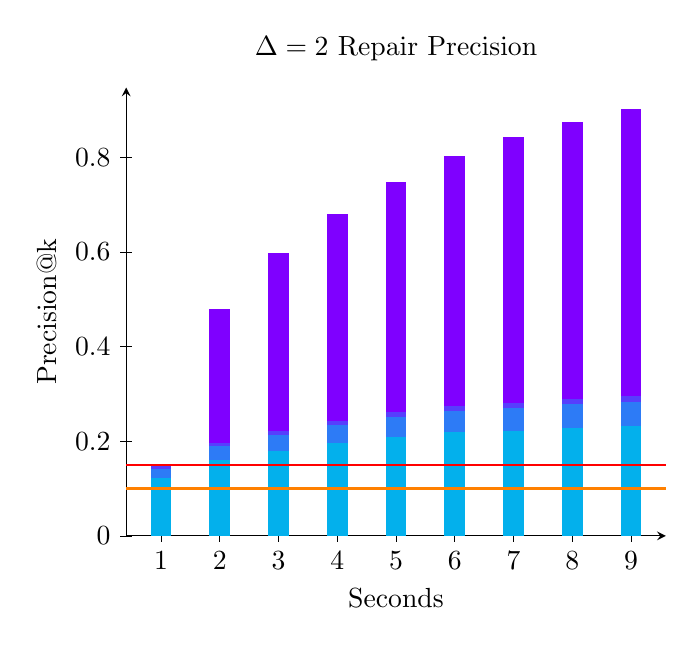
\begin{tikzpicture}
\begin{axis}[
tick align=outside,
tick pos=left,
axis lines=left,
title={\(\displaystyle \Delta=2\) Repair Precision},
x grid style={darkgray176},
xlabel={Seconds},
xmin=-0.5925, xmax=8.5925,
xtick style={color=black},
xtick={0,1,2,3,4,5,6,7,8},
xticklabels={1,2,3,4,5,6,7,8,9},
y grid style={darkgray176},
ylabel={Precision@k},
ymin=0, ymax=0.9471,
ytick style={color=black}
]
\draw[draw=none,fill=darkviolet1270255] (axis cs:0.825,0) rectangle (axis cs:1.175,0.48);
\draw[draw=none,fill=darkviolet1270255] (axis cs:1.825,0) rectangle (axis cs:2.175,0.597);
\draw[draw=none,fill=darkviolet1270255] (axis cs:2.825,0) rectangle (axis cs:3.175,0.68);
\draw[draw=none,fill=darkviolet1270255] (axis cs:3.825,0) rectangle (axis cs:4.175,0.748);
\draw[draw=none,fill=darkviolet1270255] (axis cs:4.825,0) rectangle (axis cs:5.175,0.802);
\draw[draw=none,fill=darkviolet1270255] (axis cs:5.825,0) rectangle (axis cs:6.175,0.842);
\draw[draw=none,fill=darkviolet1270255] (axis cs:6.825,0) rectangle (axis cs:7.175,0.874);
\draw[draw=none,fill=darkviolet1270255] (axis cs:7.825,0) rectangle (axis cs:8.175,0.902);
\draw[draw=none,fill=royalblue8762253] (axis cs:-0.175,0) rectangle (axis cs:0.175,0.147);

\draw[draw=none,fill=royalblue8762253] (axis cs:0.825,0) rectangle (axis cs:1.175,0.197);
\draw[draw=none,fill=royalblue8762253] (axis cs:1.825,0) rectangle (axis cs:2.175,0.221);
\draw[draw=none,fill=royalblue8762253] (axis cs:2.825,0) rectangle (axis cs:3.175,0.243);
\draw[draw=none,fill=royalblue8762253] (axis cs:3.825,0) rectangle (axis cs:4.175,0.261);
\draw[draw=none,fill=royalblue8762253] (axis cs:4.825,0) rectangle (axis cs:5.175,0.274);
\draw[draw=none,fill=royalblue8762253] (axis cs:5.825,0) rectangle (axis cs:6.175,0.281);
\draw[draw=none,fill=royalblue8762253] (axis cs:6.825,0) rectangle (axis cs:7.175,0.29);
\draw[draw=none,fill=royalblue8762253] (axis cs:7.825,0) rectangle (axis cs:8.175,0.295);
\draw[draw=none,fill=dodgerblue45123246] (axis cs:-0.175,0) rectangle (axis cs:0.175,0.142);

\draw[draw=none,fill=dodgerblue45123246] (axis cs:0.825,0) rectangle (axis cs:1.175,0.19);
\draw[draw=none,fill=dodgerblue45123246] (axis cs:1.825,0) rectangle (axis cs:2.175,0.214);
\draw[draw=none,fill=dodgerblue45123246] (axis cs:2.825,0) rectangle (axis cs:3.175,0.234);
\draw[draw=none,fill=dodgerblue45123246] (axis cs:3.825,0) rectangle (axis cs:4.175,0.251);
\draw[draw=none,fill=dodgerblue45123246] (axis cs:4.825,0) rectangle (axis cs:5.175,0.263);
\draw[draw=none,fill=dodgerblue45123246] (axis cs:5.825,0) rectangle (axis cs:6.175,0.27);
\draw[draw=none,fill=dodgerblue45123246] (axis cs:6.825,0) rectangle (axis cs:7.175,0.278);
\draw[draw=none,fill=dodgerblue45123246] (axis cs:7.825,0) rectangle (axis cs:8.175,0.283);
\draw[draw=none,fill=deepskyblue3176236] (axis cs:-0.175,0) rectangle (axis cs:0.175,0.123);

\draw[draw=none,fill=deepskyblue3176236] (axis cs:0.825,0) rectangle (axis cs:1.175,0.16);
\draw[draw=none,fill=deepskyblue3176236] (axis cs:1.825,0) rectangle (axis cs:2.175,0.18);
\draw[draw=none,fill=deepskyblue3176236] (axis cs:2.825,0) rectangle (axis cs:3.175,0.196);
\draw[draw=none,fill=deepskyblue3176236] (axis cs:3.825,0) rectangle (axis cs:4.175,0.209);
\draw[draw=none,fill=deepskyblue3176236] (axis cs:4.825,0) rectangle (axis cs:5.175,0.219);
\draw[draw=none,fill=deepskyblue3176236] (axis cs:5.825,0) rectangle (axis cs:6.175,0.222);
\draw[draw=none,fill=deepskyblue3176236] (axis cs:6.825,0) rectangle (axis cs:7.175,0.227);
\draw[draw=none,fill=deepskyblue3176236] (axis cs:7.825,0) rectangle (axis cs:8.175,0.232);
\addplot [red, thick] coordinates {(-0.8925,0.15) (14.8925,0.15)};
\addplot [orange, thick] coordinates {(-0.8925,0.10) (14.8925,0.10)};
\end{axis}

\end{tikzpicture}
}
  \resizebox{.24\textwidth}{!}{% This file was created with tikzplotlib v0.10.1.
\begin{tikzpicture}
\begin{axis}[
tick align=outside,
tick pos=left,
axis lines=left,
title={\(\displaystyle \Delta=3\) Repair Precision},
legend style={fill opacity=0.8, draw opacity=1, text opacity=1, legend columns=1, legend pos=north west},
x grid style={darkgray176},
xlabel={Seconds},
xmin=-0.5925, xmax=8.5925,
xtick style={color=black},
xtick={0,1,2,3,4,5,6,7,8},
xticklabels={10,20,30,40,50,60,70,80,90},
y grid style={darkgray176},
ylabel={Precision@k},
ymin=0, ymax=0.74655,
ytick style={color=black}
legend style={draw=none}
]
\draw[draw=none,fill=darkviolet1270255] (axis cs:0.825,0) rectangle (axis cs:1.175,0.372);
\draw[draw=none,fill=darkviolet1270255] (axis cs:1.825,0) rectangle (axis cs:2.175,0.472);
\draw[draw=none,fill=darkviolet1270255] (axis cs:2.825,0) rectangle (axis cs:3.175,0.543);
\draw[draw=none,fill=darkviolet1270255] (axis cs:3.825,0) rectangle (axis cs:4.175,0.59);
\draw[draw=none,fill=darkviolet1270255] (axis cs:4.825,0) rectangle (axis cs:5.175,0.625);
\draw[draw=none,fill=darkviolet1270255] (axis cs:5.825,0) rectangle (axis cs:6.175,0.655);
\draw[draw=none,fill=darkviolet1270255] (axis cs:6.825,0) rectangle (axis cs:7.175,0.69);
\draw[draw=none,fill=darkviolet1270255] (axis cs:7.825,0) rectangle (axis cs:8.175,0.711);
\draw[draw=none,fill=royalblue8762253] (axis cs:-0.175,0) rectangle (axis cs:0.175,0.117);

\draw[draw=none,fill=royalblue8762253] (axis cs:0.825,0) rectangle (axis cs:1.175,0.158);
\draw[draw=none,fill=royalblue8762253] (axis cs:1.825,0) rectangle (axis cs:2.175,0.204);
\draw[draw=none,fill=royalblue8762253] (axis cs:2.825,0) rectangle (axis cs:3.175,0.234);
\draw[draw=none,fill=royalblue8762253] (axis cs:3.825,0) rectangle (axis cs:4.175,0.254);
\draw[draw=none,fill=royalblue8762253] (axis cs:4.825,0) rectangle (axis cs:5.175,0.266);
\draw[draw=none,fill=royalblue8762253] (axis cs:5.825,0) rectangle (axis cs:6.175,0.273);
\draw[draw=none,fill=royalblue8762253] (axis cs:6.825,0) rectangle (axis cs:7.175,0.286);
\draw[draw=none,fill=royalblue8762253] (axis cs:7.825,0) rectangle (axis cs:8.175,0.291);
\draw[draw=none,fill=dodgerblue45123246] (axis cs:-0.175,0) rectangle (axis cs:0.175,0.111);

\draw[draw=none,fill=dodgerblue45123246] (axis cs:0.825,0) rectangle (axis cs:1.175,0.141);
\draw[draw=none,fill=dodgerblue45123246] (axis cs:1.825,0) rectangle (axis cs:2.175,0.183);
\draw[draw=none,fill=dodgerblue45123246] (axis cs:2.825,0) rectangle (axis cs:3.175,0.205);
\draw[draw=none,fill=dodgerblue45123246] (axis cs:3.825,0) rectangle (axis cs:4.175,0.223);
\draw[draw=none,fill=dodgerblue45123246] (axis cs:4.825,0) rectangle (axis cs:5.175,0.233);
\draw[draw=none,fill=dodgerblue45123246] (axis cs:5.825,0) rectangle (axis cs:6.175,0.241);
\draw[draw=none,fill=dodgerblue45123246] (axis cs:6.825,0) rectangle (axis cs:7.175,0.251);
\draw[draw=none,fill=dodgerblue45123246] (axis cs:7.825,0) rectangle (axis cs:8.175,0.256);
\draw[draw=none,fill=deepskyblue3176236] (axis cs:-0.175,0) rectangle (axis cs:0.175,0.076);

\draw[draw=none,fill=deepskyblue3176236] (axis cs:0.825,0) rectangle (axis cs:1.175,0.094);
\draw[draw=none,fill=deepskyblue3176236] (axis cs:1.825,0) rectangle (axis cs:2.175,0.113);
\draw[draw=none,fill=deepskyblue3176236] (axis cs:2.825,0) rectangle (axis cs:3.175,0.119);
\draw[draw=none,fill=deepskyblue3176236] (axis cs:3.825,0) rectangle (axis cs:4.175,0.129);
\draw[draw=none,fill=deepskyblue3176236] (axis cs:4.825,0) rectangle (axis cs:5.175,0.134);
\draw[draw=none,fill=deepskyblue3176236] (axis cs:5.825,0) rectangle (axis cs:6.175,0.138);
\draw[draw=none,fill=deepskyblue3176236] (axis cs:6.825,0) rectangle (axis cs:7.175,0.143);
\draw[draw=none,fill=deepskyblue3176236] (axis cs:7.825,0) rectangle (axis cs:8.175,0.146);
\addplot [red, thick] coordinates {(-0.8925,0.07) (14.8925,0.07)};
\addplot [orange, thick] coordinates {(-0.8925,0.04) (14.8925,0.04)};
\end{axis}

\end{tikzpicture}
}
%    \resizebox{.24\textwidth}{!}{\input{bar_hillel_repair_5}}
%\resizebox{.3\textwidth}{!}{% This file was created with tikzplotlib v0.10.1.
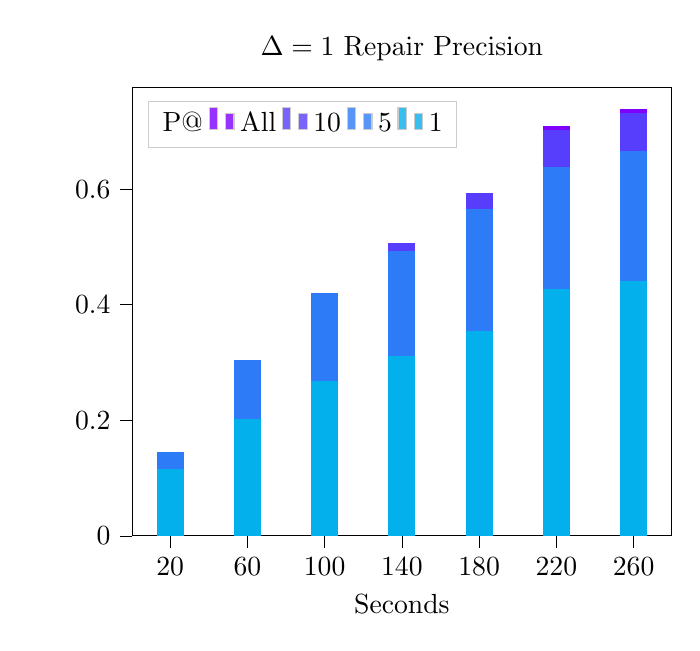
\begin{tikzpicture}

\definecolor{darkgray176}{RGB}{176,176,176}
\definecolor{darkviolet1270255}{RGB}{127,0,255}
\definecolor{deepskyblue3176236}{RGB}{3,176,236}
\definecolor{dodgerblue45123246}{RGB}{45,123,246}
\definecolor{lightgray204}{RGB}{204,204,204}
\definecolor{royalblue8762253}{RGB}{87,62,253}

\begin{axis}[
legend cell align={left},
legend style={fill opacity=0.8, draw opacity=1, text opacity=1, draw=lightgray204, legend columns=-1, legend pos=north west},
tick align=outside,
tick pos=left,
title={$\Delta=1$ Repair Precision},
x grid style={darkgray176},
xlabel={Seconds},
xmin=-0.4925, xmax=6.4925,
xtick style={color=black},
xtick={0,1,2,3,4,5,6},
xticklabels={20,60,100,140,180,220,260},
y grid style={darkgray176},
ylabel={\phantom{Precision@k}},
ymin=0, ymax=0.77595,
ytick style={color=black}
]
\addlegendimage{empty legend}
\addlegendentry{P@}
\draw[draw=none,fill=darkviolet1270255] (axis cs:-0.175,0) rectangle (axis cs:0.175,0.145);
\addlegendimage{ybar,ybar legend,draw=none,fill=darkviolet1270255}
\addlegendentry{All}

\draw[draw=none,fill=darkviolet1270255] (axis cs:0.825,0) rectangle (axis cs:1.175,0.304);
\draw[draw=none,fill=darkviolet1270255] (axis cs:1.825,0) rectangle (axis cs:2.175,0.42);
\draw[draw=none,fill=darkviolet1270255] (axis cs:2.825,0) rectangle (axis cs:3.175,0.507);
\draw[draw=none,fill=darkviolet1270255] (axis cs:3.825,0) rectangle (axis cs:4.175,0.594);
\draw[draw=none,fill=darkviolet1270255] (axis cs:4.825,0) rectangle (axis cs:5.175,0.71);
\draw[draw=none,fill=darkviolet1270255] (axis cs:5.825,0) rectangle (axis cs:6.175,0.739);
\draw[draw=none,fill=royalblue8762253] (axis cs:-0.175,0) rectangle (axis cs:0.175,0.145);
\addlegendimage{ybar,ybar legend,draw=none,fill=royalblue8762253}
\addlegendentry{10}

\draw[draw=none,fill=royalblue8762253] (axis cs:0.825,0) rectangle (axis cs:1.175,0.304);
\draw[draw=none,fill=royalblue8762253] (axis cs:1.825,0) rectangle (axis cs:2.175,0.42);
\draw[draw=none,fill=royalblue8762253] (axis cs:2.825,0) rectangle (axis cs:3.175,0.507);
\draw[draw=none,fill=royalblue8762253] (axis cs:3.825,0) rectangle (axis cs:4.175,0.594);
\draw[draw=none,fill=royalblue8762253] (axis cs:4.825,0) rectangle (axis cs:5.175,0.703);
\draw[draw=none,fill=royalblue8762253] (axis cs:5.825,0) rectangle (axis cs:6.175,0.732);
\draw[draw=none,fill=dodgerblue45123246] (axis cs:-0.175,0) rectangle (axis cs:0.175,0.145);
\addlegendimage{ybar,ybar legend,draw=none,fill=dodgerblue45123246}
\addlegendentry{5}

\draw[draw=none,fill=dodgerblue45123246] (axis cs:0.825,0) rectangle (axis cs:1.175,0.304);
\draw[draw=none,fill=dodgerblue45123246] (axis cs:1.825,0) rectangle (axis cs:2.175,0.42);
\draw[draw=none,fill=dodgerblue45123246] (axis cs:2.825,0) rectangle (axis cs:3.175,0.493);
\draw[draw=none,fill=dodgerblue45123246] (axis cs:3.825,0) rectangle (axis cs:4.175,0.565);
\draw[draw=none,fill=dodgerblue45123246] (axis cs:4.825,0) rectangle (axis cs:5.175,0.638);
\draw[draw=none,fill=dodgerblue45123246] (axis cs:5.825,0) rectangle (axis cs:6.175,0.667);
\draw[draw=none,fill=deepskyblue3176236] (axis cs:-0.175,0) rectangle (axis cs:0.175,0.116);
\addlegendimage{ybar,ybar legend,draw=none,fill=deepskyblue3176236}
\addlegendentry{1}

\draw[draw=none,fill=deepskyblue3176236] (axis cs:0.825,0) rectangle (axis cs:1.175,0.203);
\draw[draw=none,fill=deepskyblue3176236] (axis cs:1.825,0) rectangle (axis cs:2.175,0.268);
\draw[draw=none,fill=deepskyblue3176236] (axis cs:2.825,0) rectangle (axis cs:3.175,0.312);
\draw[draw=none,fill=deepskyblue3176236] (axis cs:3.825,0) rectangle (axis cs:4.175,0.355);
\draw[draw=none,fill=deepskyblue3176236] (axis cs:4.825,0) rectangle (axis cs:5.175,0.428);
\draw[draw=none,fill=deepskyblue3176236] (axis cs:5.825,0) rectangle (axis cs:6.175,0.442);
\end{axis}

\end{tikzpicture}
}
%\resizebox{.307\textwidth}{!}{% This file was created with tikzplotlib v0.10.1.
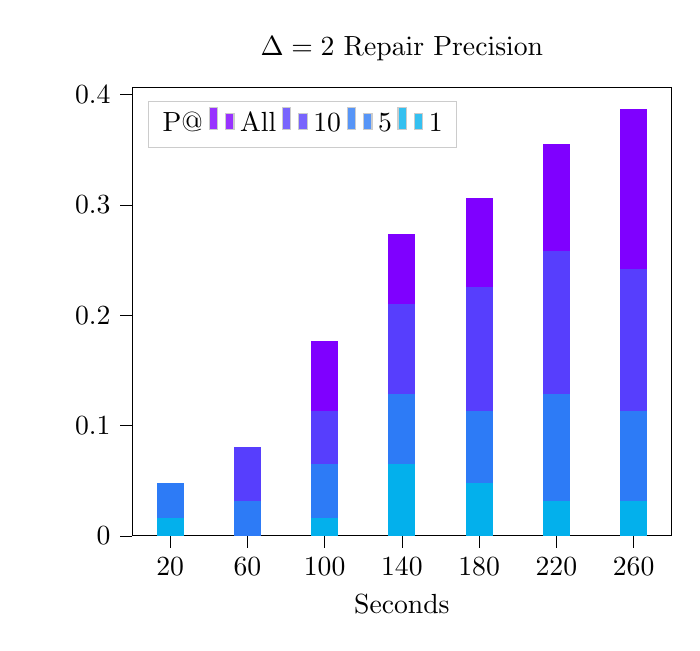
\begin{tikzpicture}

\definecolor{darkgray176}{RGB}{176,176,176}
\definecolor{darkviolet1270255}{RGB}{127,0,255}
\definecolor{deepskyblue3176236}{RGB}{3,176,236}
\definecolor{dodgerblue45123246}{RGB}{45,123,246}
\definecolor{lightgray204}{RGB}{204,204,204}
\definecolor{royalblue8762253}{RGB}{87,62,253}

\begin{axis}[
legend cell align={left},
legend style={fill opacity=0.8, draw opacity=1, text opacity=1, draw=lightgray204, legend columns=-1, legend pos=north west},
tick align=outside,
tick pos=left,
title={$\Delta=2$ Repair Precision},
x grid style={darkgray176},
xlabel={Seconds},
xmin=-0.4925, xmax=6.4925,
xtick style={color=black},
xtick={0,1,2,3,4,5,6},
xticklabels={20,60,100,140,180,220,260},
y grid style={darkgray176},
ylabel={\phantom{Precision@k}},
ymin=0, ymax=0.40635,
ytick style={color=black}
]
\addlegendimage{empty legend}
\addlegendentry{P@}
\draw[draw=none,fill=darkviolet1270255] (axis cs:-0.175,0) rectangle (axis cs:0.175,0.048);
\addlegendimage{ybar,ybar legend,draw=none,fill=darkviolet1270255}
\addlegendentry{All}

\draw[draw=none,fill=darkviolet1270255] (axis cs:0.825,0) rectangle (axis cs:1.175,0.081);
\draw[draw=none,fill=darkviolet1270255] (axis cs:1.825,0) rectangle (axis cs:2.175,0.177);
\draw[draw=none,fill=darkviolet1270255] (axis cs:2.825,0) rectangle (axis cs:3.175,0.274);
\draw[draw=none,fill=darkviolet1270255] (axis cs:3.825,0) rectangle (axis cs:4.175,0.306);
\draw[draw=none,fill=darkviolet1270255] (axis cs:4.825,0) rectangle (axis cs:5.175,0.355);
\draw[draw=none,fill=darkviolet1270255] (axis cs:5.825,0) rectangle (axis cs:6.175,0.387);
\draw[draw=none,fill=royalblue8762253] (axis cs:-0.175,0) rectangle (axis cs:0.175,0.048);
\addlegendimage{ybar,ybar legend,draw=none,fill=royalblue8762253}
\addlegendentry{10}

\draw[draw=none,fill=royalblue8762253] (axis cs:0.825,0) rectangle (axis cs:1.175,0.081);
\draw[draw=none,fill=royalblue8762253] (axis cs:1.825,0) rectangle (axis cs:2.175,0.113);
\draw[draw=none,fill=royalblue8762253] (axis cs:2.825,0) rectangle (axis cs:3.175,0.21);
\draw[draw=none,fill=royalblue8762253] (axis cs:3.825,0) rectangle (axis cs:4.175,0.226);
\draw[draw=none,fill=royalblue8762253] (axis cs:4.825,0) rectangle (axis cs:5.175,0.258);
\draw[draw=none,fill=royalblue8762253] (axis cs:5.825,0) rectangle (axis cs:6.175,0.242);
\draw[draw=none,fill=dodgerblue45123246] (axis cs:-0.175,0) rectangle (axis cs:0.175,0.048);
\addlegendimage{ybar,ybar legend,draw=none,fill=dodgerblue45123246}
\addlegendentry{5}

\draw[draw=none,fill=dodgerblue45123246] (axis cs:0.825,0) rectangle (axis cs:1.175,0.032);
\draw[draw=none,fill=dodgerblue45123246] (axis cs:1.825,0) rectangle (axis cs:2.175,0.065);
\draw[draw=none,fill=dodgerblue45123246] (axis cs:2.825,0) rectangle (axis cs:3.175,0.129);
\draw[draw=none,fill=dodgerblue45123246] (axis cs:3.825,0) rectangle (axis cs:4.175,0.113);
\draw[draw=none,fill=dodgerblue45123246] (axis cs:4.825,0) rectangle (axis cs:5.175,0.129);
\draw[draw=none,fill=dodgerblue45123246] (axis cs:5.825,0) rectangle (axis cs:6.175,0.113);
\draw[draw=none,fill=deepskyblue3176236] (axis cs:-0.175,0) rectangle (axis cs:0.175,0.016);
\addlegendimage{ybar,ybar legend,draw=none,fill=deepskyblue3176236}
\addlegendentry{1}

\draw[draw=none,fill=deepskyblue3176236] (axis cs:0.825,0) rectangle (axis cs:1.175,0);
\draw[draw=none,fill=deepskyblue3176236] (axis cs:1.825,0) rectangle (axis cs:2.175,0.016);
\draw[draw=none,fill=deepskyblue3176236] (axis cs:2.825,0) rectangle (axis cs:3.175,0.065);
\draw[draw=none,fill=deepskyblue3176236] (axis cs:3.825,0) rectangle (axis cs:4.175,0.048);
\draw[draw=none,fill=deepskyblue3176236] (axis cs:4.825,0) rectangle (axis cs:5.175,0.032);
\draw[draw=none,fill=deepskyblue3176236] (axis cs:5.825,0) rectangle (axis cs:6.175,0.032);
\end{axis}

\end{tikzpicture}
}
  \end{center}
  \caption{Latency benchmarks. Note the varying axis ranges. The red line marks Seq2Parse and the orange line marks BIFI's Precision@1.}\label{fig:human}
\end{figure}

\noindent For Precision@k, we measure the precision of our model at top-k prediction out of all instances presented, regardless of outcome. Four outcomes are possible in each repair instance, each a strict subset of the successor.

\begin{enumerate}
  \item $\textsc{Rank}(\sigma') < K$: the top-K sorted results contain the true repair
  \item $\textsc{Dec}(G_\cap) \rightsquigarrow \sigma'$: the true repair is sampled by the decoder
  \item $\sigma' \in \mathcal{L}(G_\cap)$: the true repair is recognized by the intersection grammar
  \item $|G_\cap| < \textsc{MaxHeap}:$ the intersection grammar fits in memory
\end{enumerate}

\noindent Repair cases that pass all four are the ideal, meaning the true repair was sampled and ranked highly, but often (1) fails. This indicates the decoder drew the true repair but was not able to discern its importance. Cases that fail (2) mean the decoder did not draw the true repair. In rare cases, the decoder would not have the chance to draw the true repair, as the intersection grammar is too large to represent. This typically happens when the language edit distance is very large, and the decoder is unable to fully explore all the sample space. Below, we give a summary of the repair outcomes.

\begin{figure}[H]
\begin{center}
\resizebox{.73\textwidth}{!}{% This file was created with tikzplotlib v0.10.1.
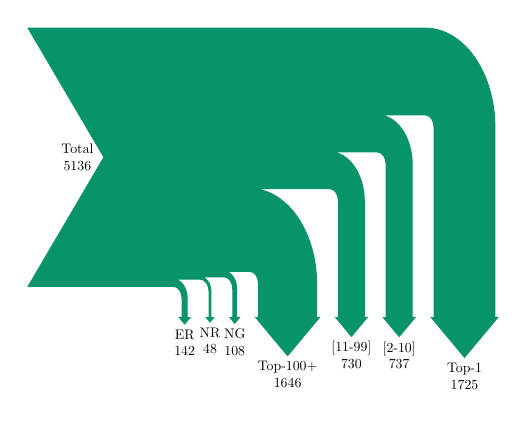
\begin{tikzpicture}

\definecolor{darkgray176}{RGB}{176,176,176}
\definecolor{teal9147104}{RGB}{9,147,104}

\begin{axis}[
hide x axis,
hide y axis,
tick align=outside,
tick pos=left,
x grid style={darkgray176},
xmin=-1.15, xmax=4.9844,
xtick style={color=black},
y grid style={darkgray176},
ymin=-2.14186236169148, ymax=1.4272,
ytick style={color=black}
]
\path [draw=teal9147104, fill=teal9147104]
(axis cs:-0.75,1.0272)
--(axis cs:-0.375,1.0272)
.. controls (axis cs:-0.09375,1.0272) and (axis cs:0.09375,1.0272) .. (axis cs:0.375,1.0272)
--(axis cs:3.7644,1.0272)
.. controls (axis cs:3.97384067067,1.0272) and (axis cs:4.17491743833,0.94391127565) .. (axis cs:4.32301435699,0.79581435699)
.. controls (axis cs:4.47111127565,0.64771743833) and (axis cs:4.5544,0.44664067067) .. (axis cs:4.5544,0.2372)
--(axis cs:4.5544,-1.2772)
--(axis cs:4.5844,-1.2772)
--(axis cs:4.2094,-1.59186236169148)
--(axis cs:3.8344,-1.2772)
--(axis cs:3.8644,-1.2772)
--(axis cs:3.8644,0.2372)
.. controls (axis cs:3.8644,0.2637114773) and (axis cs:3.8538571235,0.2891642327) .. (axis cs:3.8351106781,0.3079106781)
.. controls (axis cs:3.8163642327,0.3266571235) and (axis cs:3.7909114773,0.3372) .. (axis cs:3.7644,0.3372)
--(axis cs:3.6144,0.3372)
--(axis cs:3.2196,0.3372)
.. controls (axis cs:3.3242673123804,0.3372) and (axis cs:3.4247547906996,0.295576723578) .. (axis cs:3.4987657571388,0.2215657571388)
.. controls (axis cs:3.572776723578,0.1475547906996) and (axis cs:3.6144,0.0470673123803999) .. (axis cs:3.6144,-0.0576000000000001)
--(axis cs:3.6144,-1.2772)
--(axis cs:3.6444,-1.2772)
--(axis cs:3.467,-1.42605627457085)
--(axis cs:3.2896,-1.2772)
--(axis cs:3.3196,-1.2772)
--(axis cs:3.3196,-0.0576000000000001)
.. controls (axis cs:3.3196,-0.0310885227000001) and (axis cs:3.3090571235,-0.00563576730000012) .. (axis cs:3.2903106781,0.0131106780999999)
.. controls (axis cs:3.2715642327,0.0318571234999999) and (axis cs:3.2461114773,0.0423999999999999) .. (axis cs:3.2196,0.0423999999999999)
--(axis cs:3.0696,0.0423999999999999)
--(axis cs:2.6776,0.0423999999999999)
.. controls (axis cs:2.781524991016,0.0423999999999999) and (axis cs:2.881299792184,0.0010719241199999) .. (axis cs:2.954785858152,-0.0724141418480001)
.. controls (axis cs:3.02827192412,-0.145900207816) and (axis cs:3.0696,-0.245675008984) .. (axis cs:3.0696,-0.3496)
--(axis cs:3.0696,-1.2772)
--(axis cs:3.0996,-1.2772)
--(axis cs:2.9236,-1.4248815350872)
--(axis cs:2.7476,-1.2772)
--(axis cs:2.7776,-1.2772)
--(axis cs:2.7776,-0.3496)
.. controls (axis cs:2.7776,-0.3230885227) and (axis cs:2.7670571235,-0.2976357673) .. (axis cs:2.7483106781,-0.2788893219)
.. controls (axis cs:2.7295642327,-0.2601428765) and (axis cs:2.7041114773,-0.2496) .. (axis cs:2.6776,-0.2496)
--(axis cs:2.5276,-0.2496)
--(axis cs:1.7692,-0.2496)
.. controls (axis cs:1.9702630438432,-0.2496) and (axis cs:2.1632967407968,-0.329557175376) .. (axis cs:2.3054697827104,-0.4717302172896)
.. controls (axis cs:2.447642824624,-0.6139032592032) and (axis cs:2.5276,-0.8069369561568) .. (axis cs:2.5276,-1.008)
--(axis cs:2.5276,-1.2772)
--(axis cs:2.5576,-1.2772)
--(axis cs:2.1984,-1.57860458751888)
--(axis cs:1.8392,-1.2772)
--(axis cs:1.8692,-1.2772)
--(axis cs:1.8692,-1.008)
.. controls (axis cs:1.8692,-0.9814885227) and (axis cs:1.8586571235,-0.9560357673) .. (axis cs:1.8399106781,-0.9372893219)
.. controls (axis cs:1.8211642327,-0.9185428765) and (axis cs:1.7957114773,-0.908) .. (axis cs:1.7692,-0.908)
--(axis cs:1.6192,-0.908)
--(axis cs:1.476,-0.908)
.. controls (axis cs:1.5139644354936,-0.908) and (axis cs:1.5504127812264,-0.923097399148) .. (axis cs:1.5772576910392,-0.9499423089608)
.. controls (axis cs:1.604102600852,-0.9767872187736) and (axis cs:1.6192,-1.0132355645064) .. (axis cs:1.6192,-1.0512)
--(axis cs:1.6192,-1.2772)
--(axis cs:1.6492,-1.2772)
--(axis cs:1.5976,-1.32049754096875)
--(axis cs:1.546,-1.2772)
--(axis cs:1.576,-1.2772)
--(axis cs:1.576,-1.0512)
.. controls (axis cs:1.576,-1.0246885227) and (axis cs:1.5654571235,-0.9992357673) .. (axis cs:1.5467106781,-0.9804893219)
.. controls (axis cs:1.5279642327,-0.9617428765) and (axis cs:1.5025114773,-0.9512) .. (axis cs:1.476,-0.9512)
--(axis cs:1.326,-0.9512)
--(axis cs:1.2068,-0.9512)
.. controls (axis cs:1.2384016809416,-0.9512) and (axis cs:1.2687413653784,-0.963767108788) .. (axis cs:1.2910871282952,-0.9861128717048)
.. controls (axis cs:1.313432891212,-1.0084586346216) and (axis cs:1.326,-1.0387983190584) .. (axis cs:1.326,-1.0704)
--(axis cs:1.326,-1.2772)
--(axis cs:1.356,-1.2772)
--(axis cs:1.3164,-1.31042834539462)
--(axis cs:1.2768,-1.2772)
--(axis cs:1.3068,-1.2772)
--(axis cs:1.3068,-1.0704)
.. controls (axis cs:1.3068,-1.0438885227) and (axis cs:1.2962571235,-1.0184357673) .. (axis cs:1.2775106781,-0.9996893219)
.. controls (axis cs:1.2587642327,-0.9809428765) and (axis cs:1.2333114773,-0.9704) .. (axis cs:1.2068,-0.9704)
--(axis cs:1.0568,-0.9704)
--(axis cs:0.9,-0.9704)
.. controls (axis cs:0.9415699964064,-0.9704) and (axis cs:0.9814799168736,-0.986931230352) .. (axis cs:1.0108743432608,-1.0163256567392)
.. controls (axis cs:1.040268769648,-1.0457200831264) and (axis cs:1.0568,-1.0856300035936) .. (axis cs:1.0568,-1.1272)
--(axis cs:1.0568,-1.2772)
--(axis cs:1.0868,-1.2772)
--(axis cs:1.0284,-1.32620341846075)
--(axis cs:0.97,-1.2772)
--(axis cs:1,-1.2772)
--(axis cs:1,-1.1272)
.. controls (axis cs:1,-1.1006885227) and (axis cs:0.9894571235,-1.0752357673) .. (axis cs:0.9707106781,-1.0564893219)
.. controls (axis cs:0.9519642327,-1.0377428765) and (axis cs:0.9265114773,-1.0272) .. (axis cs:0.9,-1.0272)
--(axis cs:0.75,-1.0272)
--(axis cs:0.75,-1.0272)
--(axis cs:0.375,-1.0272)
.. controls (axis cs:0.09375,-1.0272) and (axis cs:-0.09375,-1.0272) .. (axis cs:-0.375,-1.0272)
--(axis cs:-0.75,-1.0272)
--(axis cs:-0.75,-1.0272)
--(axis cs:0.111923141145302,0)
--(axis cs:-0.75,1.0272)
--(axis cs:-0.5,1.0272)
--(axis cs:-0.75,1.0272)
--cycle;
\draw (axis cs:-0.038076858854698,0) node[
  scale=0.5,
  text=black,
  rotate=0.0,
  align=center
]{Total\phantom{.......}\\5136\phantom{.......}};
\draw (axis cs:4.2094,-1.74186236169148) node[
  scale=0.5,
  text=black,
  rotate=0.0,
  align=center
]{Top-1\\1725};
\draw (axis cs:3.467,-1.57605627457085) node[
  scale=0.5,
  text=black,
  rotate=0.0,
  align=center
]{[2-10]\\737};
\draw (axis cs:2.9236,-1.5748815350872) node[
  scale=0.5,
  text=black,
  rotate=0.0,
  align=center
]{[11-99]\\730};
\draw (axis cs:2.1984,-1.72860458751888) node[
  scale=0.5,
  text=black,
  rotate=0.0,
  align=center
]{Top-100+\\1646};
\draw (axis cs:1.5976,-1.47049754096875) node[
  scale=0.5,
  text=black,
  rotate=0.0,
  align=center
]{NG\\108};
\draw (axis cs:1.3164,-1.46042834539462) node[
  scale=0.5,
  text=black,
  rotate=0.0,
  align=center
]{NR\\48};
\draw (axis cs:1.0284,-1.47620341846075) node[
  scale=0.5,
  text=black,
  rotate=0.0,
  align=center
]{ER\\142};
\end{axis}

\end{tikzpicture}
}
\caption{Summarized repair outcomes from the SO Python dataset. (ER=Error, NR=Not recognized, NG=Not generated). Time: $\sim$10h on M1.}
\end{center}
\end{figure}
